% !TeX root = ../main.tex
\chapter{Resolución numérica de ecuaciones diferenciales difusas}
\begin{chapquote}{Conversación entre Katherine Johnson \& John Glenn, \textit{Figuras ocultas}}
	John Glenn: ``Pasar de una trayectoria elíptica a otra parabólica`` \\
	Katherine Johnson: ``No se trata de una solución teórica, sino numérica`` \cite{eulernasa}
\end{chapquote}

En esta sección se van a ver diferentes técnicas para resolver ecuaciones diferenciales difusas, abarcando desde las técnicas clásicas de la resolución númerica de ecuaciones diferenciales hasta las técnicas más sofisticadas a nivel computacional.

En esta sección se va a hacer un análisis exhaustivo en las ventajas que nos ofrecen los distintos métodos con vistas a obtener el rendimiento más óptimo en cuánto a velocidad y en eficiencia enerǵetica.

Para entender esta sección sería conveniente revisar algunas de las técnicas mostradas en la sección anterior, y repasar las tećnicas básicas de resolución numérica de ecuaciones diferenciales difusas.

\section{El método de Euler}
En esta sección se va a desarrollar el método de Euler para problemas difusos, para ello se empieza recordando como funciona el método de Euler para ecuaciones diferenciales ordinales.

\subsection{Método de Euler: Versión clásica}
Se supone que se tiene un problema de valores iniciales bien definido, y lo suficiente regular para asegurar que tiene soluciones:
\[
\begin{array}{ccc}
	y' & = &f(x, y)  \\
	y(x_0) & = & y_0
\end{array}
\]
Se considera ahora una discretación de $x$ de manera que:
\[
	x_i = x_0 + i h
\]
Donde $h$ se llama paso del método de Euler, entonces se define la discretización de $y$ como:
\[
	y_{i+1} = y_i + h f(x_i, y_i)
\]
La definición de $y_{i+1}$ se llama Método de Euler.

\subsection{Método de Euler: Versión difusa}
Se considera el siguiente problema difuso,
\[
	\begin{array}{ccc}
		y' & = &f(x, y)  \\
		y(x_0) & = & A
	\end{array}
\]
Donde $A$ es un número difuso, se supone que el problema anterior cumple el \hyperref[teorema:equivalencia]{Teorema de equivalencia entre EDO y EDD}, y se considera el problema determinista asociado:
\[
	\begin{array}{ccc}
		y' & = &f(x, y)  \\
		y(x_0) & = & a
	\end{array}
\]
Donde $a \in A$, se toma entonces $A$ como una discretización de $n+1$ elementos de $A$, donde cada elemento se denota por $a_i$, por tanto se tienen ahora $n+1$ EDO diferentes, donde cada una de estas se pueden resolver aplicando el método de Euler.
\subsection{Método de Euler: Ejemplo}
\begin{ejemplo}
Dado un problema de valores iniciales difuso:
\[
y' = 2x - 3y + 1
\]
\[
y(0) = (-1;0;1)
\]
Claramente cumple las hipótesis del \hyperref[teorema:equivalencia]{Teorema de equivalencia entre EDO y EDD}, por tanto el problema determinista asociado es:
\[
y' = 2x - 3y + 1
\]
\[
y(0) = a
\]

Con $a \in [-1, 1]$. \\
En primer lugar, hay que discretizar el intervalo $[-1, 1]$, para ello se considera una partición dada por 
\[
a_i = -1 + \frac{2i}{m-1}
\]

Teniendo en cuenta estas particiones, se puede aproximar la solución del problema difuso resolviendo las $m$ ecuaciones diferenciales que se deducen al tomar:

\[
y' = 2x - 3y + 1
\]
\[
y(0) = a_i
\]

Se construye ahora el método de Euler para la ecuación asociada a $a_i$ con tamaño del paso $h$, sea $x_0=0$ y tomemos $y_0 = a_i$, siguiendo entonces con le definición del método nos queda:
\[
y_{j+1} = y_j + h (2x_j - 3y_j + 1)
\]
\[
x_{j+1} = x_0 + hj
\]

Para comparar el error de nuestro método, tengamos en cuenta:
\[
y_i(x) = \frac{e^{-3 x} (-1 + 9 a_i + e^{3 x}(1 + 6 x))}{9}
\]
A continuación, se ofrecerá varías implementaciones del método con información descriptiva acerca del rendimiento energético y en tiempo:

\subsection{Experimentos numéricos}
Se va a tratar de resolver el problema anterior aplicando el método de Euler, con una implementación en C y otra en Python, donde se varía la cantidad de particiones del número difuso triangular y con 100 pasos en el método de Euler.
\subsubsection{Implementación en Python}
\begin{figure}[H]
	\frame{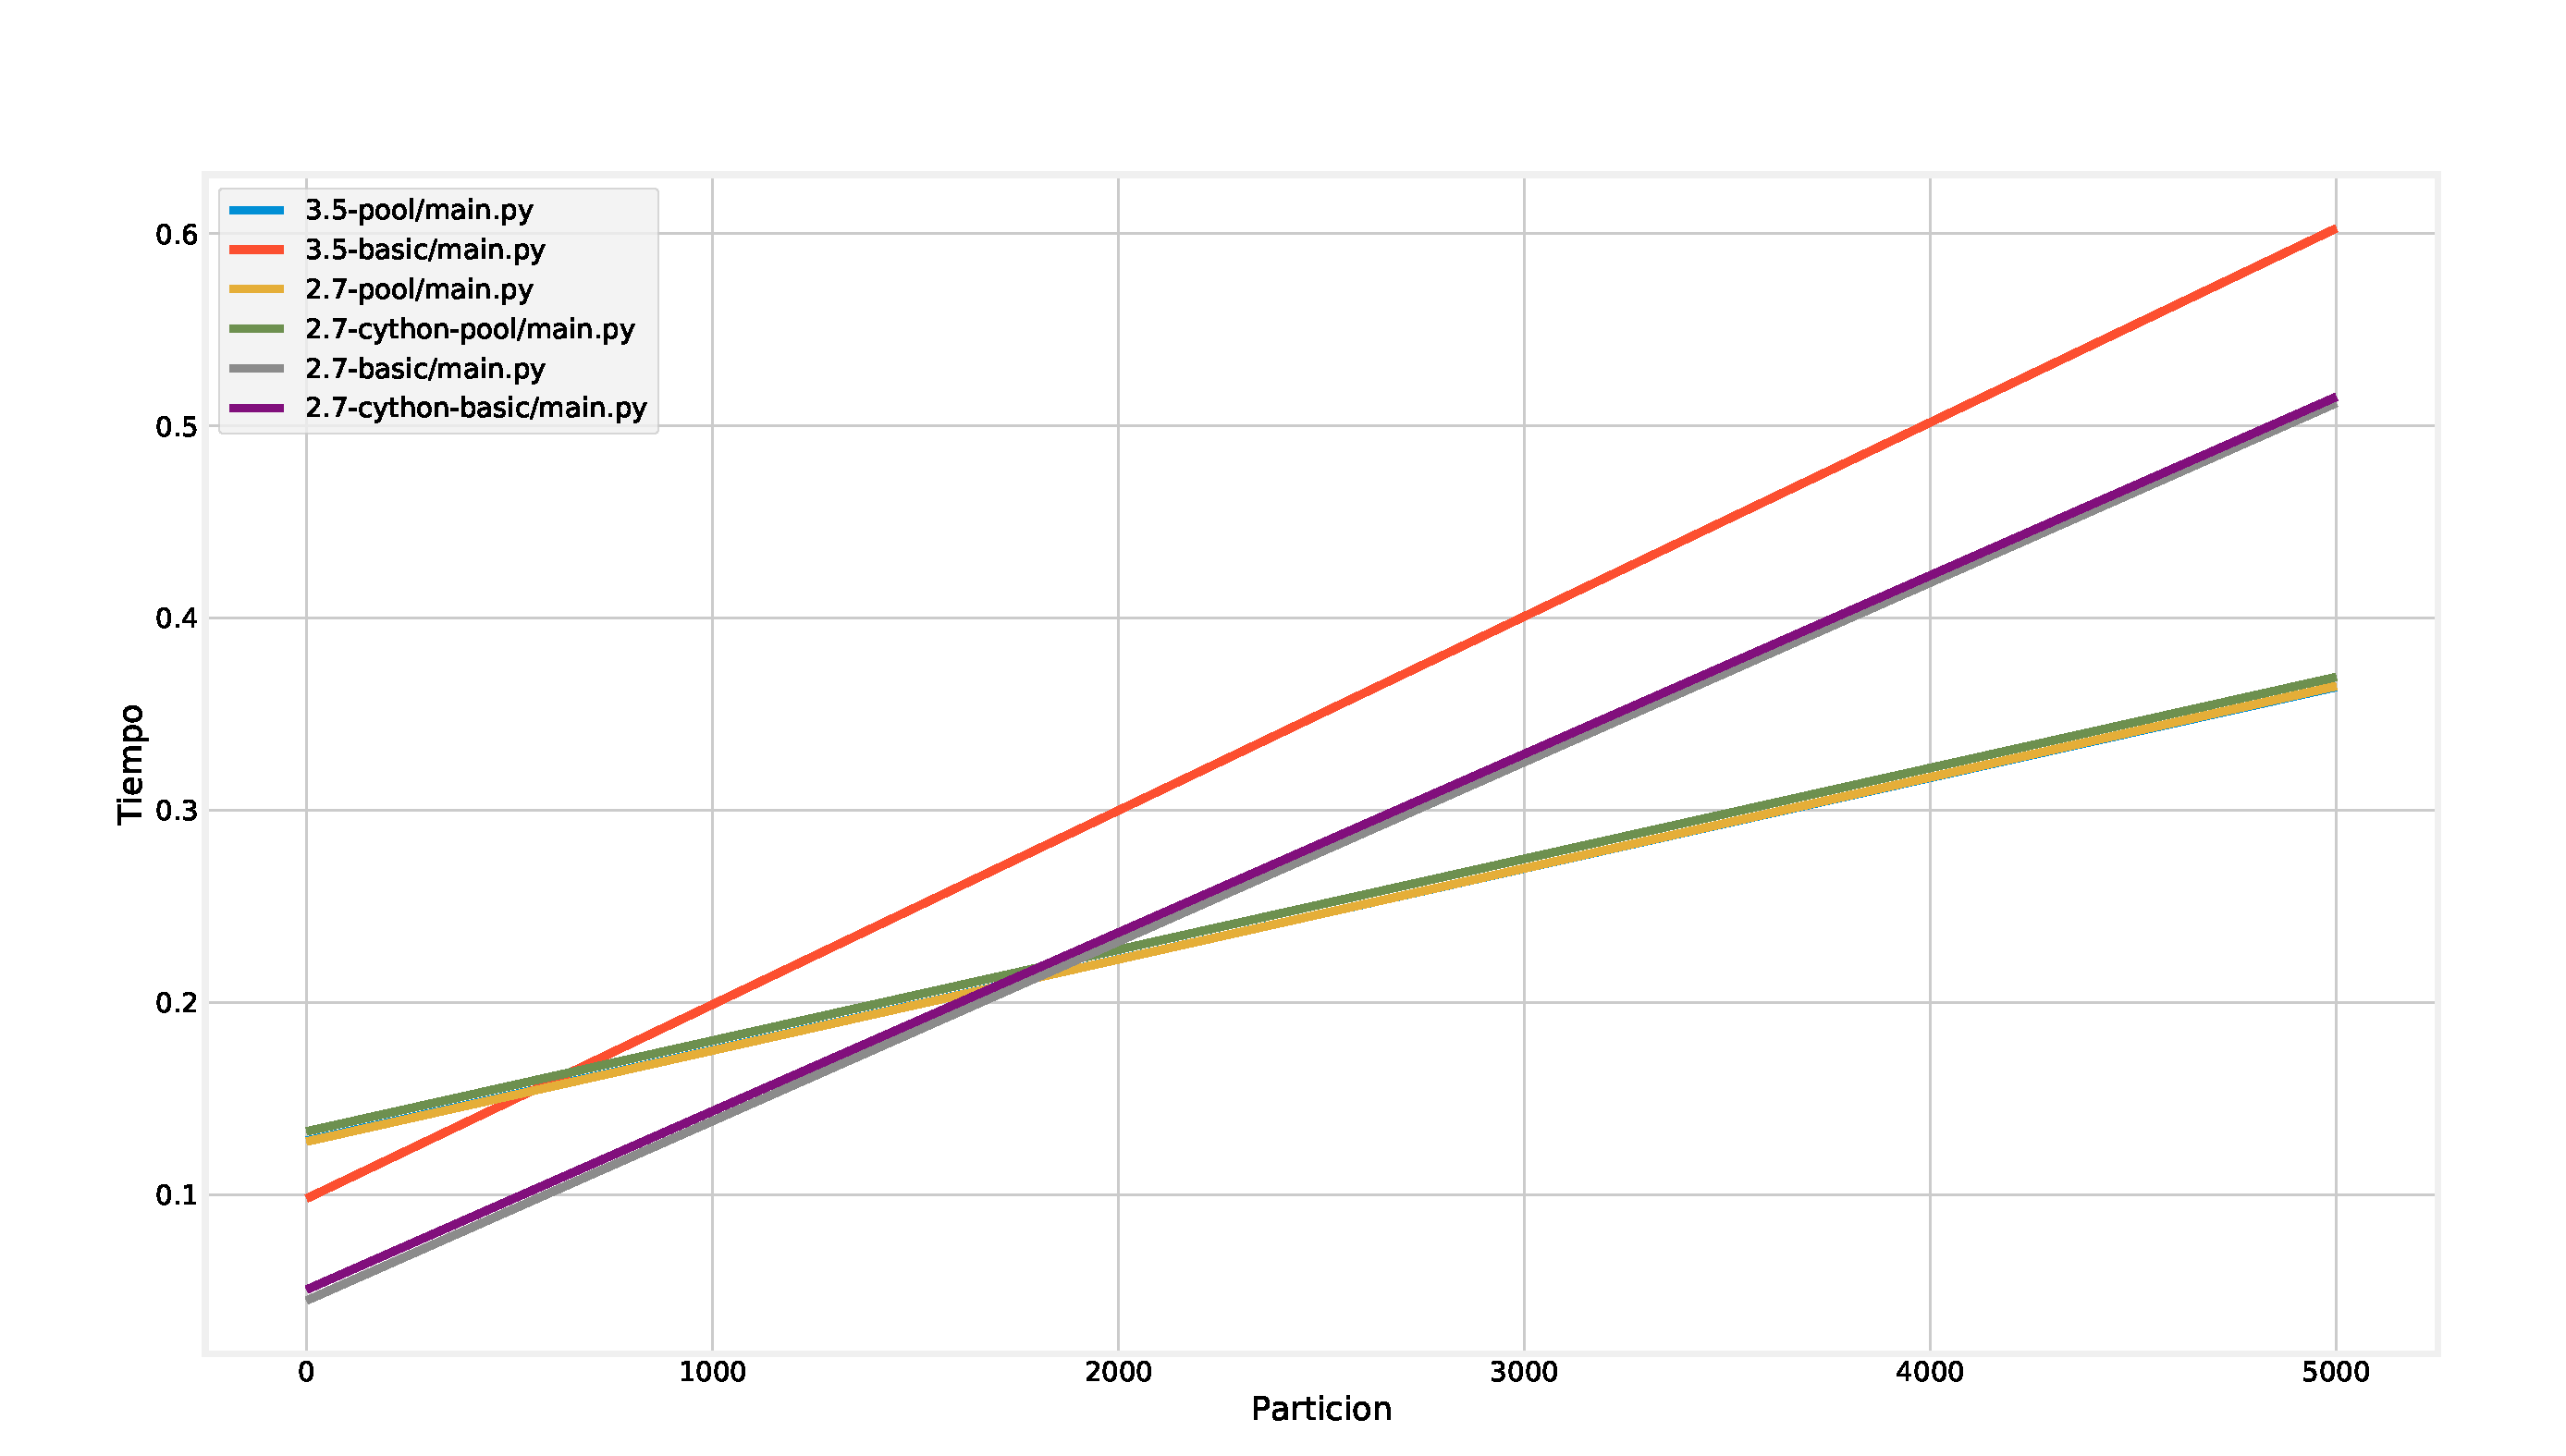
\includegraphics[width=\textwidth]{grafica_python_euler_comparativa.pdf}}
	\centering
	\caption{Distintos resultados en Python}
	\label{fig:eulerpython}
\end{figure}

Se pueden observar, varios patrones:

\begin{itemize}
	\item La forma menos eficiente de resolver el problema es usando una versión más reciente de Python.
	\item Trabajar con Cython no nos asegura un rendimiento mejor.
	\item El crecimiento del tiempo de ejecución en paralelo crece mucho más lento que en secuencial.
	\item Si se quiere resolver un problema pequeño $(n < 2000)$ es conveniente hacerlo de manera secuencial.
\end{itemize}

A continuación, se muestra una tabla con los resultados obtenidos por cada test.
\begin{table}[H]
	\centering
	\begin{tabular}{|c|c|}
		\hline
		\textbf{Test}  & \textbf{Tiempo}        \\ \hline
		2.7 Paralelo   & 61 minutos    \\
		3.5 Paralelo   & 61 minutos   \\
		2.7 Cython     & 85 minutos    \\
		2.7 Secuencial & 85.22 minutos \\ 
		3.5 Secuencial & 100 minutos   \\
		\hline
	\end{tabular}%
\end{table}
\subsubsection{Implementación en C: Secuencial}
\begin{figure}[H]
	\frame{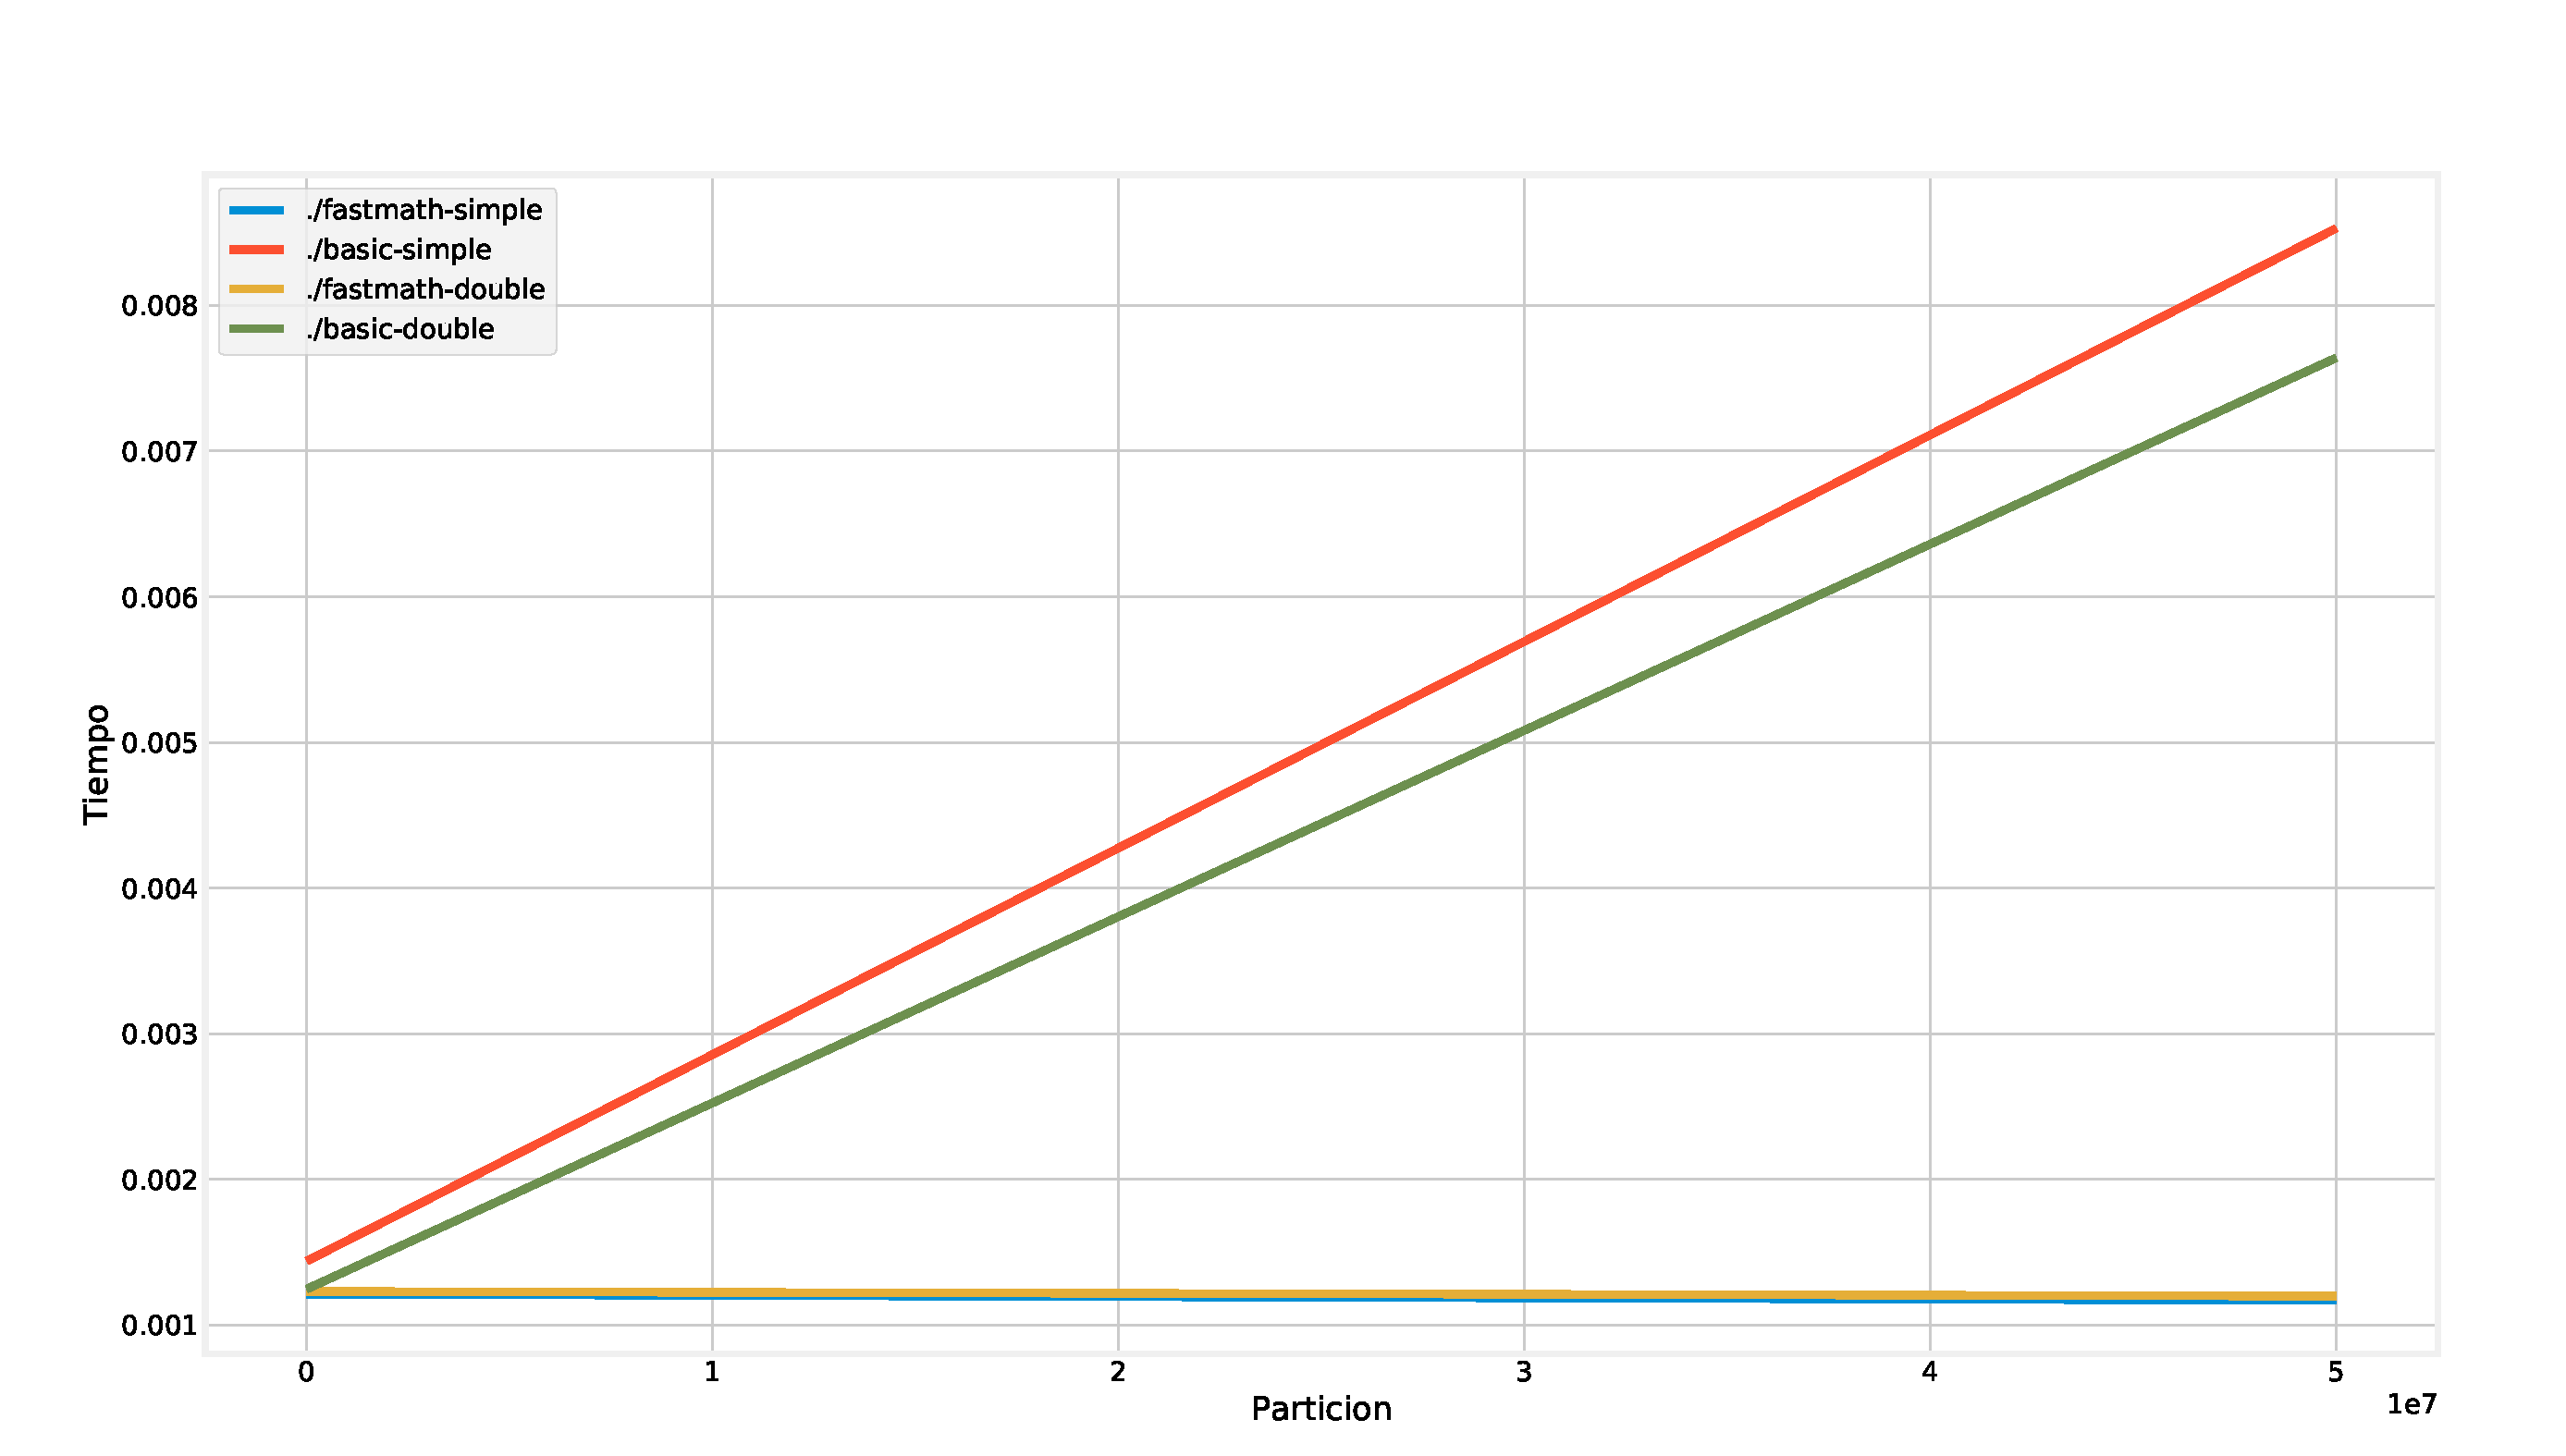
\includegraphics[width=\textwidth]{grafica_cseq_euler_comparativa.pdf}}
	\centering
	\caption{Distintos resultados en C}
	\label{fig:eulercseq}
\end{figure}
En esta parte se va a probar una implementación en C, usando diferentes técnicas numéricas.
\begin{itemize}
	\item Se han obtenido resultados esperados en las compilaciones básicas de los programas.
	\item Cuando se trabaja en doble precisión, el rendimiento se reduce, pero en C se siguen consiguiendo resultados bastantes rápidos independientemente de la precisión.
	\item El consumo de RAM es bastante reducido.
	\item El procesador al ser un procesador de 64 bits, trabaja mejor en doble precisión que en simple precisión.
\end{itemize}

A continuación, se muestra una tabla con los resultados obtenidos por cada test.

\begin{table}[H]
	\centering
	\begin{tabular}{|c|c|}
		\hline
		\textbf{Test}  & \textbf{Tiempo}        \\ \hline
		Fastmath simple & 11.9 segundos \\ 
		Fastmath doble   & 12.15 segundos    \\
		Doble   & 75.80 segundos \\
		Simple     & 85 segundos    \\
		\hline
	\end{tabular}%
\end{table}

Ahora vamos a ver que sucede si también se aumenta el número de particiones para representar el número difuso, y para obtener resultados más interesantes, se van a empezar las iteraciones en 10000.

\begin{figure}[H]
	\frame{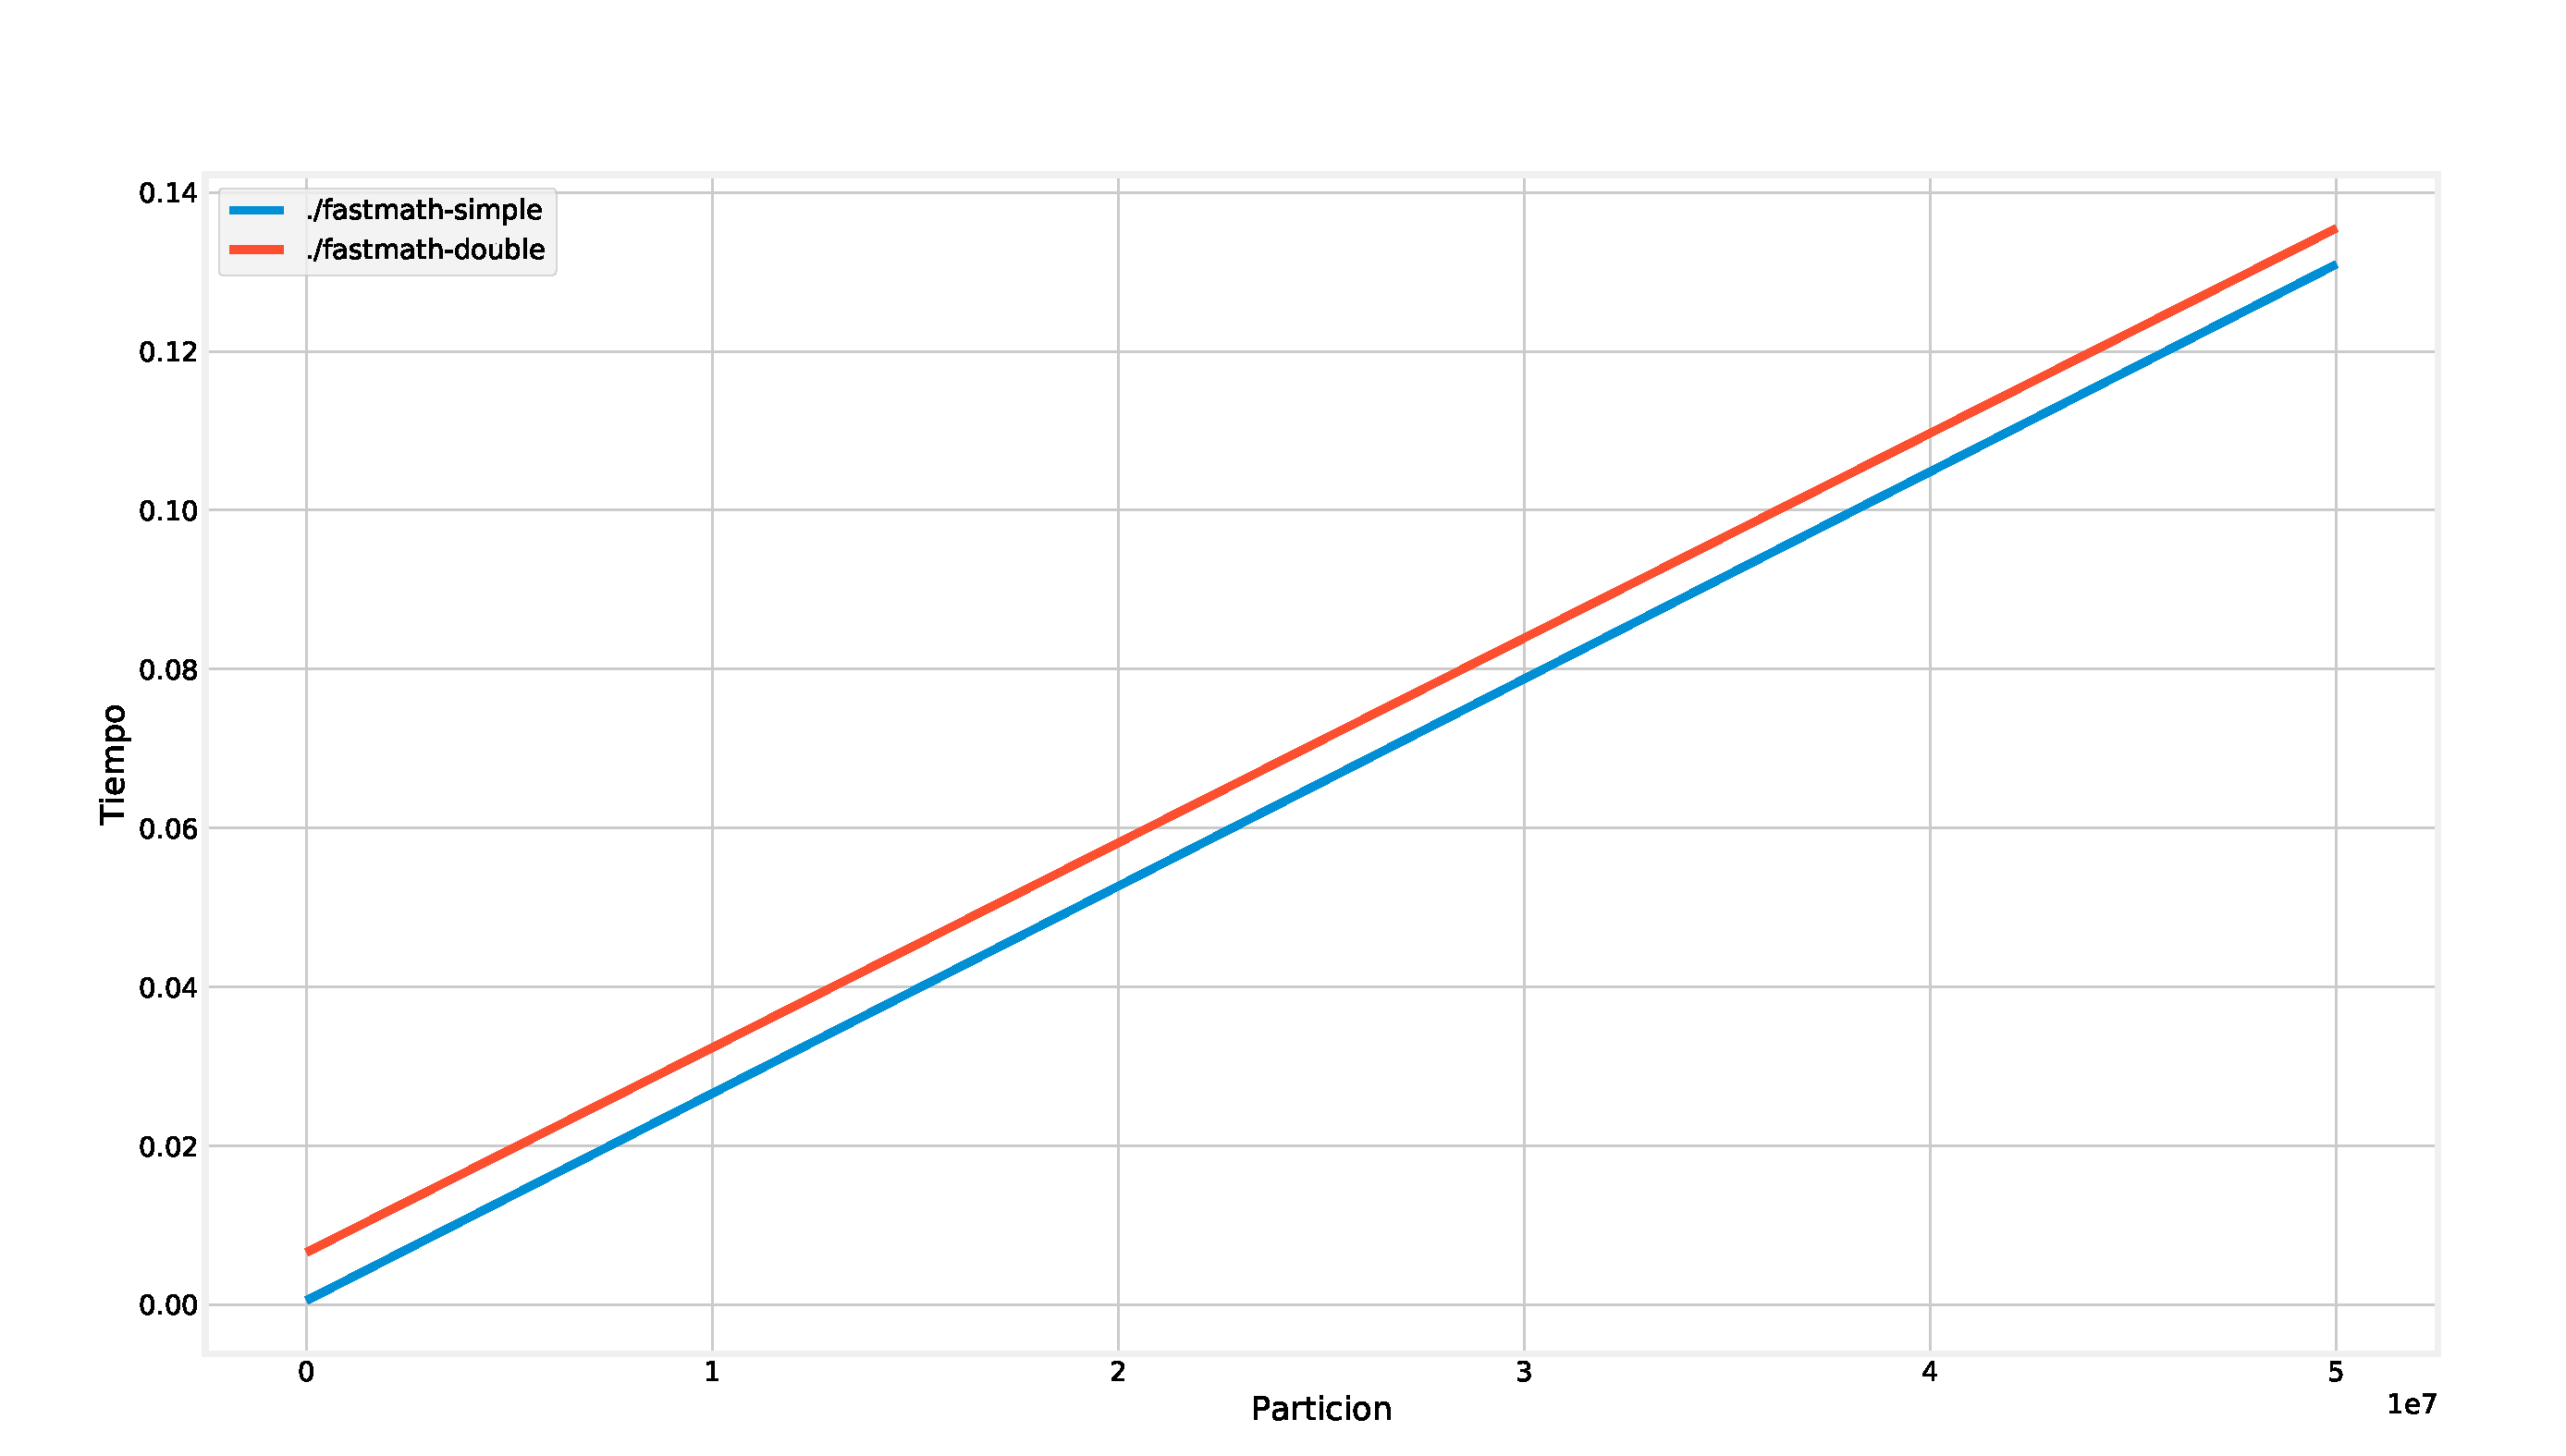
\includegraphics[width=\textwidth]{grafica_cseq_euler_comparativa_2.pdf}}
	\centering
	\caption{Distintos resultados en C}
	\label{fig:eulercseq2}
\end{figure}
Aquí se pueden sacar una conclusiones diferentes,
\begin{enumerate}
	\item Es más óptimo trabajar en simple precisión con fastmath.
	
	\item Pese a todo, aunque se esté haciendo $10^{16}$ iteraciones, el algoritmo tarda como mucho $0.25$ segundos, aún no es necesario plantearse trabajar en paralelo.
\end{enumerate}
Finalmente, se introduce una tabla con los tiempos de cada prueba

\begin{table}[H]
	\centering
	\begin{tabular}{|c|c|}
		\hline
		\textbf{Test}  & \textbf{Tiempo}        \\ \hline
		Fastmath simple & 1278.03 segundos \\ 
		Fastmath doble   & 1341.10 segundos  \\ \hline
	\end{tabular}%
\end{table}

Por otro lado, en la siguiente tabla se muestran los consumo energético de los distintos ejemplos para $10^{5}$ iteraciones.

\begin{table}[H]
	\centering
	\begin{tabular}{|c|c|}
		\hline
		\textbf{Test}  & \textbf{Consumo energético}        \\ \hline
		Fastmath simple & $118.644028 \mu A/s$ \\ 
		Fastmath doble   & $118.644058 \mu A/s$ \\
		Simple & $ 152.542389 \mu A/s$ \\
		Doble & $ 169.491638 \mu A/s$ \\
		\hline
	\end{tabular}%
\end{table}
\subsubsection{Conclusiones}
En contra de lo que se pueda pensar comúnmente, trabajar con precisión doble es más eficiente en procesadores modernos de 64 bits que trabajar en precisión simple, así que no hay que tener miedo a trabajar con doble precisión. \\
Los resultados obtenidos en C con la flag -OFast son sorprendentes, tan sorprendentes que no se ha planteado la necesidad  de implementar el método en paralelo por la eficiencia de aplicar esa flag.
\\
Y no sólo permite obtener una solución numérica más rápidamente, sino que permite consumir menos recursos energéticos, lo que se traduce en un ahorro económico a la hora de trabajar a una escala mayor, y un menor impacto medioambiental, por tanto utilizar la flag -Ofast al compilar es la mejor opción en todos los aspectos
\end{ejemplo}

\section{Método de Runge-Kutta}
\subsubsection{Implementación en C: Secuencial}
\subsubsection{Implementación en C: Paralelo}
\subsubsection{Implementación en CUDA}
\subsubsection{Conclusiones}

\section{Comparativas}